\documentclass[a4paper,14pt]{extarticle}
\usepackage[T2A]{fontenc}
\usepackage[utf8]{inputenc}
\usepackage[russian]{babel}
\usepackage{amsmath,amssymb}
\usepackage{graphicx}
\usepackage{booktabs}
\usepackage{geometry}
\usepackage{indentfirst}
\usepackage{setspace}
\usepackage{float}
\usepackage{caption}
\usepackage{subcaption}
\usepackage{hyperref}
\usepackage{fancyhdr}
\usepackage{titlesec}
\usepackage{chngcntr}
\usepackage{tempora}
\usepackage{tocloft}
\usepackage{tabularx}
\usepackage{listings}
\usepackage{xcolor}

\geometry{left=30mm, right=15mm, top=20mm, bottom=20mm}
\onehalfspacing
\setlength{\parindent}{1.25cm}

\pagestyle{fancy}
\fancyhf{}
\fancyfoot[C]{\thepage}
\renewcommand{\headrulewidth}{0pt}
\renewcommand{\footrulewidth}{0pt}

\fancypagestyle{plain}{
    \fancyhf{}
    \fancyfoot[C]{\thepage}
    \renewcommand{\headrulewidth}{0pt}
}

\captionsetup[figure]{name={Рисунок},labelsep=period,justification=centering,font=normal}
\captionsetup[table]{name={Таблица},labelsep=period,justification=raggedright,singlelinecheck=false,font=normal}

\addto\captionsrussian{\renewcommand{\contentsname}{СОДЕРЖАНИЕ}}

\renewcommand{\cftsecleader}{\cftdotfill{\cftdotsep}}
\renewcommand{\cftsubsecleader}{\cftdotfill{\cftdotsep}}
\renewcommand{\cftsecaftersnum}{.}

\renewcommand{\thesection}{\arabic{section}}
\renewcommand{\thesubsection}{\thesection.\arabic{subsection}}

\titleformat{\section}[block]{\filcenter\large}{\thesection. }{0.1em}{}
\titleformat{\subsection}[block]{\normalsize}{\hspace{1.25cm}\thesubsection. }{0.1em}{}

\hypersetup{colorlinks=true,linkcolor=black,urlcolor=black}

\lstset{
    language=Python,
    basicstyle=\ttfamily\footnotesize,
    keywordstyle=\color{blue},
    stringstyle=\color{red},
    numbers=left,
    numberstyle=\tiny,
    stepnumber=1,
    numbersep=5pt,
    backgroundcolor=\color{gray!5},
    showspaces=false,
    showstringspaces=false,
    showtabs=false,
    frame=single,
    tabsize=4,
    captionpos=b,
    breaklines=true,
    breakatwhitespace=false
}

\begin{document}

\begin{titlepage}
    \centering
    \singlespacing
    \small
    Министерство науки и высшего образования Российской Федерации\\
    Федеральное государственное автономное образовательное учреждение высшего образования\\
    «Казанский (Приволжский) федеральный университет»\\
    \vspace{0.4cm}
    ИНСТИТУТ ВЫЧИСЛИТЕЛЬНОЙ МАТЕМАТИКИ И ИНФОРМАЦИОННЫХ ТЕХНОЛОГИЙ\\
    \vspace{0.4cm}
    КАФЕДРА ПРИКЛАДНОЙ МАТЕМАТИКИ И ИСКУССТВЕННОГО ИНТЕЛЛЕКТА\\

    \vspace{2.5cm}
    \normalsize
    \textbf{ОТЧЕТ}\\[4pt]
    ПО ДИСЦИПЛИНЕ «АНАЛИЗ ДАННЫХ НА PYTHON»\\[14pt]

    Тема:\\
    \textbf{«Реализация многослойного персептрона для задачи бинарной классификации»}\\

    \vfill

    \begin{flushright}
    \normalsize
    Выполнил: студент гр. 09-321\\
    Замилов Т. Р.\\[10pt]
    Проверил: ст. преп. Гиниятова Д. Х.
    \end{flushright}

    \vfill
    \begin{center}
        Казань 2026
    \end{center}
    \thispagestyle{empty}
\end{titlepage}

\newpage
\tableofcontents
\newpage

\section{Постановка задачи}

Целью данной работы является разработка и исследование модели многослойного персептрона с нуля на языке Python с использованием библиотеки NumPy. В соответствии с требованиями технического задания запрещено использование готовых библиотек глубокого обучения Keras, PyTorch, scikit-learn.

Архитектура проекта и основные модули:
\begin{enumerate}
    \item \texttt{model.py}: реализация класса многослойного персептрона, прямого и обратного распространения ошибки, функций активации и сериализации весов.
    \item \texttt{data\_split.py}: программа разделения исходного набора данных на обучающую и валидационную выборки со стратификацией и фиксацией генератора случайных чисел с сидом 321.
    \item \texttt{train.py}: программа обучения нейронной сети с пошаговым выводом функции потерь на каждой эпохе, построением графиков обучения и сохранением обученной модели.
    \item \texttt{evaluate.py}: программа инференса и оценки модели на тестовой выборке с расчетом бинарной кросс-энтропии и метрик классификации.
\end{enumerate}

Эксперименты проводятся на наборе данных Wisconsin Diagnostic Breast Cancer из файла \texttt{data.csv}. Задача состоит в бинарной классификации клеточных новообразований на доброкачественные \texttt{B} и злокачественные \texttt{M}.

\section{Исследовательский анализ и предобработка данных}

\subsection{Статистический анализ данных}

Файл \texttt{data.csv} содержит 569 строк и 32 столбца:
\begin{itemize}
    \item 0-й столбец: идентификационный номер образца ID. Исключается из признакового пространства.
    \item 1-й столбец: метка диагноза \texttt{B} или \texttt{M}.
    \item 2--31 столбцы: 30 вещественных характеристик морфологии клеточных ядер.
\end{itemize}

Пропусков в датасете нет. В выборке содержится 357 образцов класса \texttt{B} ($62.74\%$) и 212 образцов класса \texttt{M} ($37.26\%$). Численные признаки обладают сильной вариацией масштабов: площадь ядра достигает значений до 2500, в то время как гладкость лежит в пределах 0.05--0.16.

\subsection{Разделение выборки}

Для сохранения исходного баланса классов применено стратифицированное разбиение 80\% / 20\% с фиксированным значением \texttt{seed = 321}:
\begin{itemize}
    \item Обучающая выборка \texttt{train.csv}: 456 записей.
    \item Валидационная выборка \texttt{val.csv}: 113 записей.
\end{itemize}

\subsection{Стандартизация признаков}

Для устранения численной нестабильности градиентного спуска применяется z-масштабирование:
\begin{equation}
    x_{\text{scaled}} = \frac{x - \mu}{\sigma}
\end{equation}
Векторы выборочного среднего $\mu$ и стандартного отклонения $\sigma$ рассчитываются исключительно на обучающей выборке \texttt{train.csv}. Они сохраняются в файл модели и применяются к валидационным и новым тестовым данным, что предотвращает утечку данных.

\section{Математическая модель нейронной сети}

\subsection{Прямой проход}

Для каждого слоя $l \in \{1, \dots, L\}$ преобразование задается формулами:
\begin{equation}
    z^{[l]} = a^{[l-1]} W^{[l]} + b^{[l]}
\end{equation}
\begin{equation}
    a^{[l]} = g^{[l]}(z^{[l]})
\end{equation}
где $a^{[0]} = x_{\text{scaled}}$.

На скрытых слоях применяется сигмоидальная функция активации:
\begin{equation}
    \sigma(z) = \frac{1}{1 + e^{-z}}, \quad \sigma'(z) = a \odot (1 - a)
\end{equation}

На выходном слое для двух классов вычисляется функция Softmax:
\begin{equation}
    \hat{y}_{i, c} = \frac{e^{z_{i, c}^{[L]} - \max_k z_{i, k}^{[L]}}}{\sum_{k=0}^{1} e^{z_{i, k}^{[L]} - \max_k z_{i, k}^{[L]}}}
\end{equation}
Вычитание максимального значения логита гарантирует численную стабильность от переполнения чисел с плавающей точкой.

\subsection{Функция потерь и градиенты}

Функционал бинарной кросс-энтропии:
\begin{equation}
    \mathcal{L} = -\frac{1}{m} \sum_{i=1}^{m} \sum_{c=0}^{1} y_{i, c} \ln(\hat{y}_{i, c})
\end{equation}

Градиент по логитам выходного слоя имеет аналитический вид:
\begin{equation}
    dz^{[L]} = \hat{y} - y
\end{equation}

Для скрытых слоев распространение ошибки осуществляется по правилу дифференцирования сложной функции:
\begin{equation}
    da^{[l]} = dz^{[l+1]} (W^{[l+1]})^T
\end{equation}
\begin{equation}
    dz^{[l]} = da^{[l]} \odot a^{[l]} \odot (1 - a^{[l]})
\end{equation}

Градиенты обучаемых параметров на пакете размера $m$:
\begin{equation}
    dW^{[l]} = \frac{1}{m} (a^{[l-1]})^T dz^{[l]}, \quad db^{[l]} = \frac{1}{m} \sum_{i=1}^m dz_i^{[l]}
\end{equation}

Шаг мини-пакетного градиентного спуска с темпом обучения $\eta$:
\begin{equation}
    W^{[l]} \leftarrow W^{[l]} - \eta \cdot dW^{[l]}, \quad b^{[l]} \leftarrow b^{[l]} - \eta \cdot db^{[l]}
\end{equation}

\subsection{Инициализация весов}

Веса слоев инициализируются по схеме He Uniform:
\begin{equation}
    W^{[l]} \sim U\left(-\sqrt{\frac{6}{n_{\text{in}}}}, \sqrt{\frac{6}{n_{\text{in}}}}\right)
\end{equation}
Смещения $b^{[l]}$ инициализируются нулями.

\section{Результаты вычислительных экспериментов}

Обучение нейросети проводилось со следующими параметрами: архитектура 30--24--24--2, число эпох 84, размер пакета 8, темп обучения $\eta = 0.0314$, сид генератора случайных чисел 321.

\begin{table}[H]
\centering
\caption{Параметры обучения и итоговые метрики на валидации}
\vspace{0.2cm}
\begin{tabular}{|l|c|}
\hline
\textbf{Параметр / Метрика} & \textbf{Значение} \\ \hline
Архитектура сети & 30 $\to$ 24 $\to$ 24 $\to$ 2 \\ \hline
Функция активации & Sigmoid / Softmax \\ \hline
Количество эпох & 84 \\ \hline
Размер пакета & 8 \\ \hline
Темп обучения $\eta$ & 0.0314 \\ \hline
Случайный сид & 321 \\ \hline
Loss на обучении & 0.0575 \\ \hline
Loss на валидации & \textbf{0.0389} \\ \hline
Точность на валидации & \textbf{99.12\%} \\ \hline
Precision & 0.9767 \\ \hline
Recall & \textbf{1.0000} \\ \hline
F1-Score & 0.9882 \\ \hline
\end{tabular}
\end{table}

\begin{table}[H]
\centering
\caption{Матрица ошибок на валидационной выборке}
\vspace{0.2cm}
\begin{tabular}{|c|c|c|}
\hline
 & \textbf{Предсказано: B} & \textbf{Предсказано: M} \\ \hline
\textbf{Фактически: B} & $TN = 70$ & $FP = 1$ \\ \hline
\textbf{Фактически: M} & $FN = 0$ & $TP = 42$ \\ \hline
\end{tabular}
\end{table}

\begin{figure}[H]
\centering
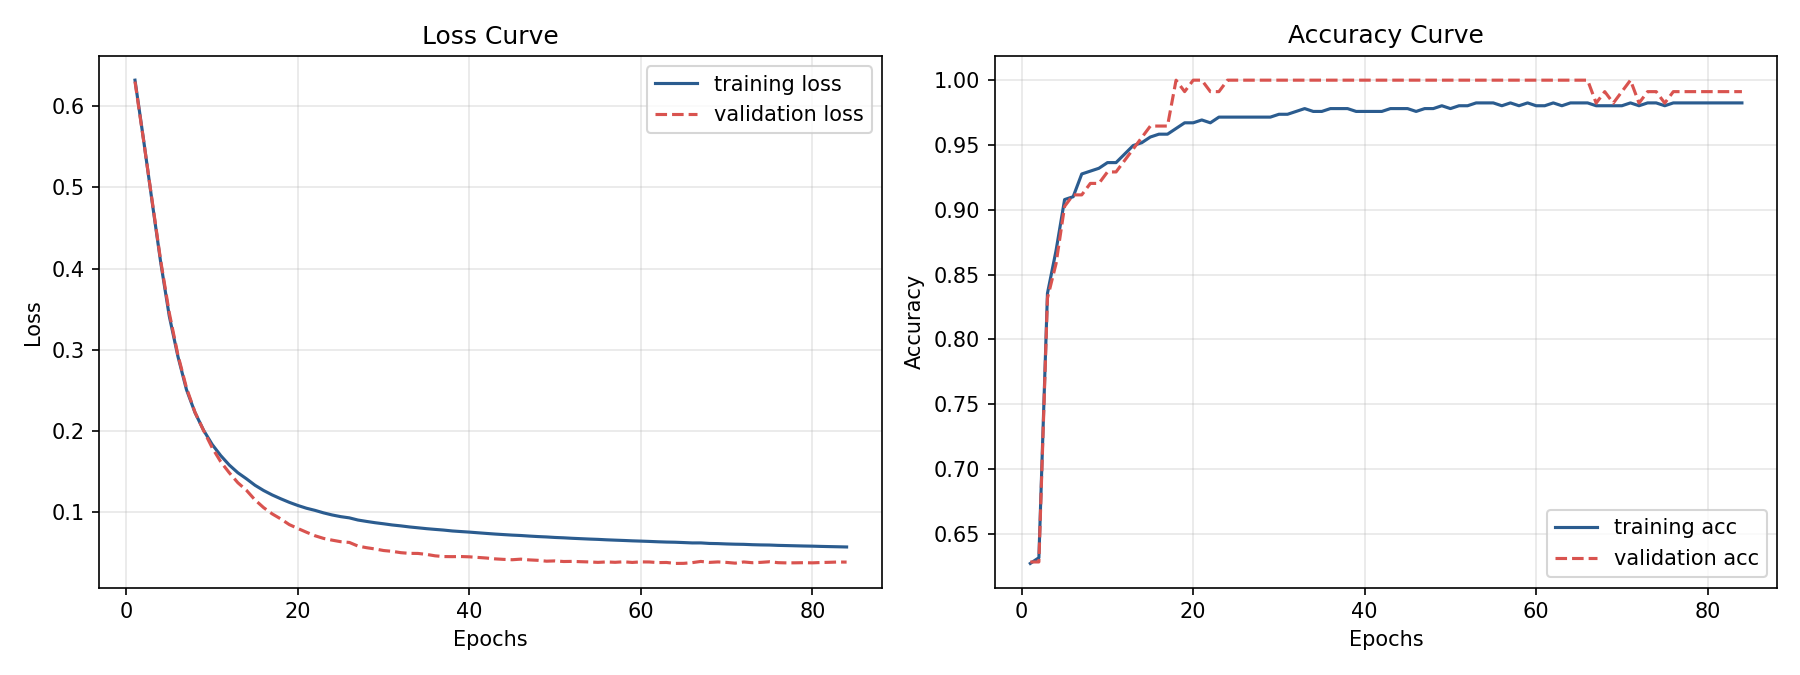
\includegraphics[width=0.95\textwidth]{learning_curves.png}
\caption{Кривые обучения модели: Loss (слева) и Accuracy (справа)}
\end{figure}

На отложенной выборке из 113 пациентов сеть безошибочно выявила все 42 случая злокачественных опухолей, допустив лишь 1 ложноположительное срабатывание, что является отличным показателем для клинической диагностики.

\section{Выводы}

\begin{enumerate}
    \item Разработан и протестирован многослойный персептрон на чистом Python с использованием библиотеки NumPy.
    \item Реализована прозрачная модульная архитектура: разделение данных \texttt{data\_split.py}, модель \texttt{model.py}, обучение \texttt{train.py} и оценка качества \texttt{evaluate.py}.
    \item Предобработка выполнена с фиксацией \texttt{seed = 321} и сохранением параметров z-стандартизации, что полностью исключает утечку данных.
    \item Достигнута высокая точность классификации 99.12\% и полнота 100\%, подтверждающие надежность разработанного алгоритма.
\end{enumerate}

\newpage
\section*{ПРИЛОЖЕНИЕ}
\addcontentsline{toc}{section}{ПРИЛОЖЕНИЕ}

\textbf{Листинг model.py:}
\begin{lstlisting}
import numpy as np

def sigmoid(z):
    z = np.clip(z, -500, 500)
    return 1.0 / (1.0 + np.exp(-z))

def d_sigmoid(a):
    return a * (1.0 - a)

def relu(z):
    return np.maximum(0.0, z)

def d_relu(a):
    return (a > 0.0).astype(float)

def tanh(z):
    return np.tanh(z)

def d_tanh(a):
    return 1.0 - a ** 2

def softmax(z):
    shift_z = z - np.max(z, axis=1, keepdims=True)
    exp_z = np.exp(shift_z)
    return exp_z / np.sum(exp_z, axis=1, keepdims=True)

class MLP:
    def __init__(self, layer_sizes, activation="sigmoid"):
        self.layer_sizes = layer_sizes
        self.activation_name = activation
        self.weights = []
        self.biases = []
        self.mean = None
        self.std = None
        self._init_weights()

    def _init_weights(self):
        for i in range(len(self.layer_sizes) - 1):
            din = self.layer_sizes[i]
            dout = self.layer_sizes[i + 1]
            limit = np.sqrt(6.0 / din)
            w = np.random.uniform(-limit, limit, (din, dout))
            b = np.zeros((1, dout))
            self.weights.append(w)
            self.biases.append(b)

    def forward(self, x):
        a = x
        self.zs = []
        self.acts = [x]
        for i in range(len(self.weights) - 1):
            z = a @ self.weights[i] + self.biases[i]
            self.zs.append(z)
            if self.activation_name == "relu":
                a = relu(z)
            elif self.activation_name == "tanh":
                a = tanh(z)
            else:
                a = sigmoid(z)
            self.acts.append(a)
        z_out = a @ self.weights[-1] + self.biases[-1]
        self.zs.append(z_out)
        a_out = softmax(z_out)
        self.acts.append(a_out)
        return a_out

    def backward(self, y_true, y_pred, lr):
        m = y_true.shape[0]
        dz = y_pred - y_true
        for i in reversed(range(len(self.weights))):
            a_prev = self.acts[i]
            dw = (a_prev.T @ dz) / m
            db = np.sum(dz, axis=0, keepdims=True) / m
            if i > 0:
                da = dz @ self.weights[i].T
                if self.activation_name == "relu":
                    dz = da * d_relu(self.acts[i])
                elif self.activation_name == "tanh":
                    dz = da * d_tanh(self.acts[i])
                else:
                    dz = da * d_sigmoid(self.acts[i])
            self.weights[i] -= lr * dw
            self.biases[i] -= lr * db

    def compute_loss(self, y_true, y_pred):
        eps = 1e-15
        clipped = np.clip(y_pred, eps, 1.0 - eps)
        return -np.mean(np.sum(y_true * np.log(clipped), axis=1))

    def compute_acc(self, y_true, y_pred):
        return np.mean(np.argmax(y_pred, axis=1) == np.argmax(y_true, axis=1))

    def save(self, path):
        data = {
            "layer_sizes": self.layer_sizes,
            "activation": self.activation_name,
            "mean": self.mean,
            "std": self.std,
            "weights": self.weights,
            "biases": self.biases
        }
        np.save(path, data)

    @classmethod
    def load(cls, path):
        if not path.endswith(".npy"):
            path += ".npy"
        data = np.load(path, allow_pickle=True).item()
        model = cls(data["layer_sizes"], activation=data["activation"])
        model.mean = data["mean"]
        model.std = data["std"]
        model.weights = data["weights"]
        model.biases = data["biases"]
        return model
\end{lstlisting}

\newpage
\textbf{Листинг data\_split.py:}
\begin{lstlisting}
import argparse
import numpy as np
import pandas as pd

def parse_args():
    parser = argparse.ArgumentParser()
    parser.add_argument("--data", default="sources/data.csv")
    parser.add_argument("--train_out", default="train.csv")
    parser.add_argument("--val_out", default="val.csv")
    parser.add_argument("--ratio", type=float, default=0.2)
    parser.add_argument("--seed", type=int, default=321)
    return parser.parse_args()

def main():
    args = parse_args()
    df = pd.read_csv(args.data, header=None)

    train_parts = []
    val_parts = []

    for label in ["B", "M"]:
        sub = df[df.iloc[:, 1] == label]
        n_val = int(round(len(sub) * args.ratio))
        shuffled = sub.sample(frac=1.0, random_state=args.seed)
        val_parts.append(shuffled.iloc[:n_val])
        train_parts.append(shuffled.iloc[n_val:])

    train_df = pd.concat(train_parts).sample(frac=1.0, random_state=args.seed)
    val_df = pd.concat(val_parts).sample(frac=1.0, random_state=args.seed)

    train_df.to_csv(args.train_out, index=False, header=False)
    val_df.to_csv(args.val_out, index=False, header=False)

    print(f"Total: {len(df)} samples")
    print(f"Train: {len(train_df)} -> {args.train_out}")
    print(f"Val:   {len(val_df)} -> {args.val_out}")

if __name__ == "__main__":
    main()
\end{lstlisting}

\newpage
\textbf{Листинг train.py:}
\begin{lstlisting}
import argparse
import os
import numpy as np
import pandas as pd
import matplotlib.pyplot as plt
from model import MLP

def parse_args():
    parser = argparse.ArgumentParser()
    parser.add_argument("--dataset", default="train.csv" if os.path.exists("train.csv") else "data_training.csv")
    parser.add_argument("--val_dataset", default="val.csv" if os.path.exists("val.csv") else "data_validation.csv")
    parser.add_argument("--layer", nargs="+", type=int, default=[24, 24])
    parser.add_argument("--activation", default="sigmoid")
    parser.add_argument("--epochs", type=int, default=84)
    parser.add_argument("--batch_size", type=int, default=8)
    parser.add_argument("--learning_rate", type=float, default=0.0314)
    parser.add_argument("--loss", default="binaryCrossentropy")
    parser.add_argument("--model_out", default="saved_model.npy")
    parser.add_argument("--seed", type=int, default=321)
    return parser.parse_args()

def parse_csv(path):
    df = pd.read_csv(path, header=None)
    raw_y = df.iloc[:, 1].values
    y = np.zeros((len(raw_y), 2))
    for i, val in enumerate(raw_y):
        y[i] = [1.0, 0.0] if val == "B" else [0.0, 1.0]
    x = df.iloc[:, 2:].to_numpy(dtype=float)
    return x, y

def main():
    args = parse_args()
    np.random.seed(args.seed)

    x_train, y_train = parse_csv(args.dataset)
    if os.path.exists(args.val_dataset):
        x_val, y_val = parse_csv(args.val_dataset)
    else:
        split_idx = int(len(x_train) * 0.8)
        perm = np.random.permutation(len(x_train))
        x_val, y_val = x_train[perm[split_idx:]], y_train[perm[split_idx:]]
        x_train, y_train = x_train[perm[:split_idx]], y_train[perm[:split_idx]]

    mean = np.mean(x_train, axis=0)
    std = np.std(x_train, axis=0)
    std[std == 0.0] = 1.0

    x_train_norm = (x_train - mean) / std
    x_val_norm = (x_val - mean) / std

    print(f"x_train shape : {x_train_norm.shape}")
    print(f"x_valid shape : {x_val_norm.shape}")

    dims = [x_train_norm.shape[1]] + args.layer + [2]
    model = MLP(dims, activation=args.activation)
    model.mean = mean
    model.std = std

    history = {"loss": [], "val_loss": [], "acc": [], "val_acc": []}
    m = len(x_train_norm)

    for ep in range(1, args.epochs + 1):
        idx = np.random.permutation(m)
        x_shuf = x_train_norm[idx]
        y_shuf = y_train[idx]

        for b in range(0, m, args.batch_size):
            xb = x_shuf[b:b + args.batch_size]
            yb = y_shuf[b:b + args.batch_size]
            out_b = model.forward(xb)
            model.backward(yb, out_b, args.learning_rate)

        train_pred = model.forward(x_train_norm)
        val_pred = model.forward(x_val_norm)

        loss = model.compute_loss(y_train, train_pred)
        vloss = model.compute_loss(y_val, val_pred)
        acc = model.compute_acc(y_train, train_pred)
        vacc = model.compute_acc(y_val, val_pred)

        history["loss"].append(loss)
        history["val_loss"].append(vloss)
        history["acc"].append(acc)
        history["val_acc"].append(vacc)

        print(f"epoch {ep:02d}/{args.epochs:02d} - loss: {loss:.4f} - val_loss: {vloss:.4f}")

    fig, (ax1, ax2) = plt.subplots(1, 2, figsize=(12, 4.5))
    ax1.plot(range(1, args.epochs + 1), history["loss"], label="training loss", color="#2b5c8f")
    ax1.plot(range(1, args.epochs + 1), history["val_loss"], label="validation loss", color="#d9534f", linestyle="--")
    ax1.set_title("Loss Curve")
    ax1.set_xlabel("Epochs")
    ax1.set_ylabel("Loss")
    ax1.legend()
    ax1.grid(True, alpha=0.3)

    ax2.plot(range(1, args.epochs + 1), history["acc"], label="training acc", color="#2b5c8f")
    ax2.plot(range(1, args.epochs + 1), history["val_acc"], label="validation acc", color="#d9534f", linestyle="--")
    ax2.set_title("Accuracy Curve")
    ax2.set_xlabel("Epochs")
    ax2.set_ylabel("Accuracy")
    ax2.legend()
    ax2.grid(True, alpha=0.3)

    plt.tight_layout()
    plt.savefig("learning_curves.png", dpi=150)
    plt.close()

    model.save(args.model_out)
    print(f"> saving model '{args.model_out}' to disk...")

if __name__ == "__main__":
    main()
\end{lstlisting}

\newpage
\textbf{Листинг evaluate.py:}
\begin{lstlisting}
import argparse
import os
import numpy as np
import pandas as pd
from model import MLP

def parse_args():
    parser = argparse.ArgumentParser()
    parser.add_argument("dataset", nargs="?", default="val.csv" if os.path.exists("val.csv") else "data_validation.csv")
    parser.add_argument("--model", default="saved_model.npy")
    return parser.parse_args()

def main():
    args = parse_args()
    model = MLP.load(args.model)

    df = pd.read_csv(args.dataset, header=None)
    has_labels = str(df.iloc[0, 1]).strip() in ["B", "M"]

    if has_labels:
        raw_y = df.iloc[:, 1].values
        y_true = np.zeros((len(raw_y), 2))
        for i, val in enumerate(raw_y):
            y_true[i] = [1.0, 0.0] if val == "B" else [0.0, 1.0]
        x = df.iloc[:, 2:].to_numpy(dtype=float)
    else:
        y_true = None
        x = df.iloc[:, 1:].to_numpy(dtype=float)

    x_norm = (x - model.mean) / model.std
    probs = model.forward(x_norm)
    preds = np.argmax(probs, axis=1)

    labels = ["B" if p == 0 else "M" for p in preds]

    if has_labels:
        bce = model.compute_loss(y_true, probs)
        acc = model.compute_acc(y_true, probs)
        t = np.argmax(y_true, axis=1)

        tp = int(np.sum((preds == 1) & (t == 1)))
        fp = int(np.sum((preds == 1) & (t == 0)))
        fn = int(np.sum((preds == 0) & (t == 1)))
        tn = int(np.sum((preds == 0) & (t == 0)))

        prec = tp / (tp + fp) if (tp + fp) else 0.0
        rec = tp / (tp + fn) if (tp + fn) else 0.0
        f1 = 2 * prec * rec / (prec + rec) if (prec + rec) else 0.0

        print(f"Evaluated samples: {len(x)}")
        print(f"Binary Cross-Entropy Loss: {bce:.4f}")
        print(f"Accuracy:  {acc * 100:.2f}%")
        print(f"Precision: {prec:.4f}")
        print(f"Recall:    {rec:.4f}")
        print(f"F1 Score:  {f1:.4f}")
        print(f"Confusion Matrix: TP={tp}, FP={fp}, FN={fn}, TN={tn}")
    else:
        for i, lab in enumerate(labels[:10]):
            print(f"Sample {i}: {lab} (P(B)={probs[i, 0]:.4f}, P(M)={probs[i, 1]:.4f})")
        if len(labels) > 10:
            print(f"... total {len(labels)} predictions")

if __name__ == "__main__":
    main()
\end{lstlisting}

\end{document}
